%=================================================================
\section{Introduction}\label{sec-intro}
\subsection{Problem Statement}
The competation \textit{Google QUEST Q\&A Labeling} is designed to 
improving automated understanding of complex question answer content.
The challenge is to use this new dataset to build predictive algorithms for different subjective aspects of question-answering. 
The question-answer pairs were gathered from nearly 70 different websites, in a "common-sense" fashion.
\begin{figure}[htbp]
    \centering
    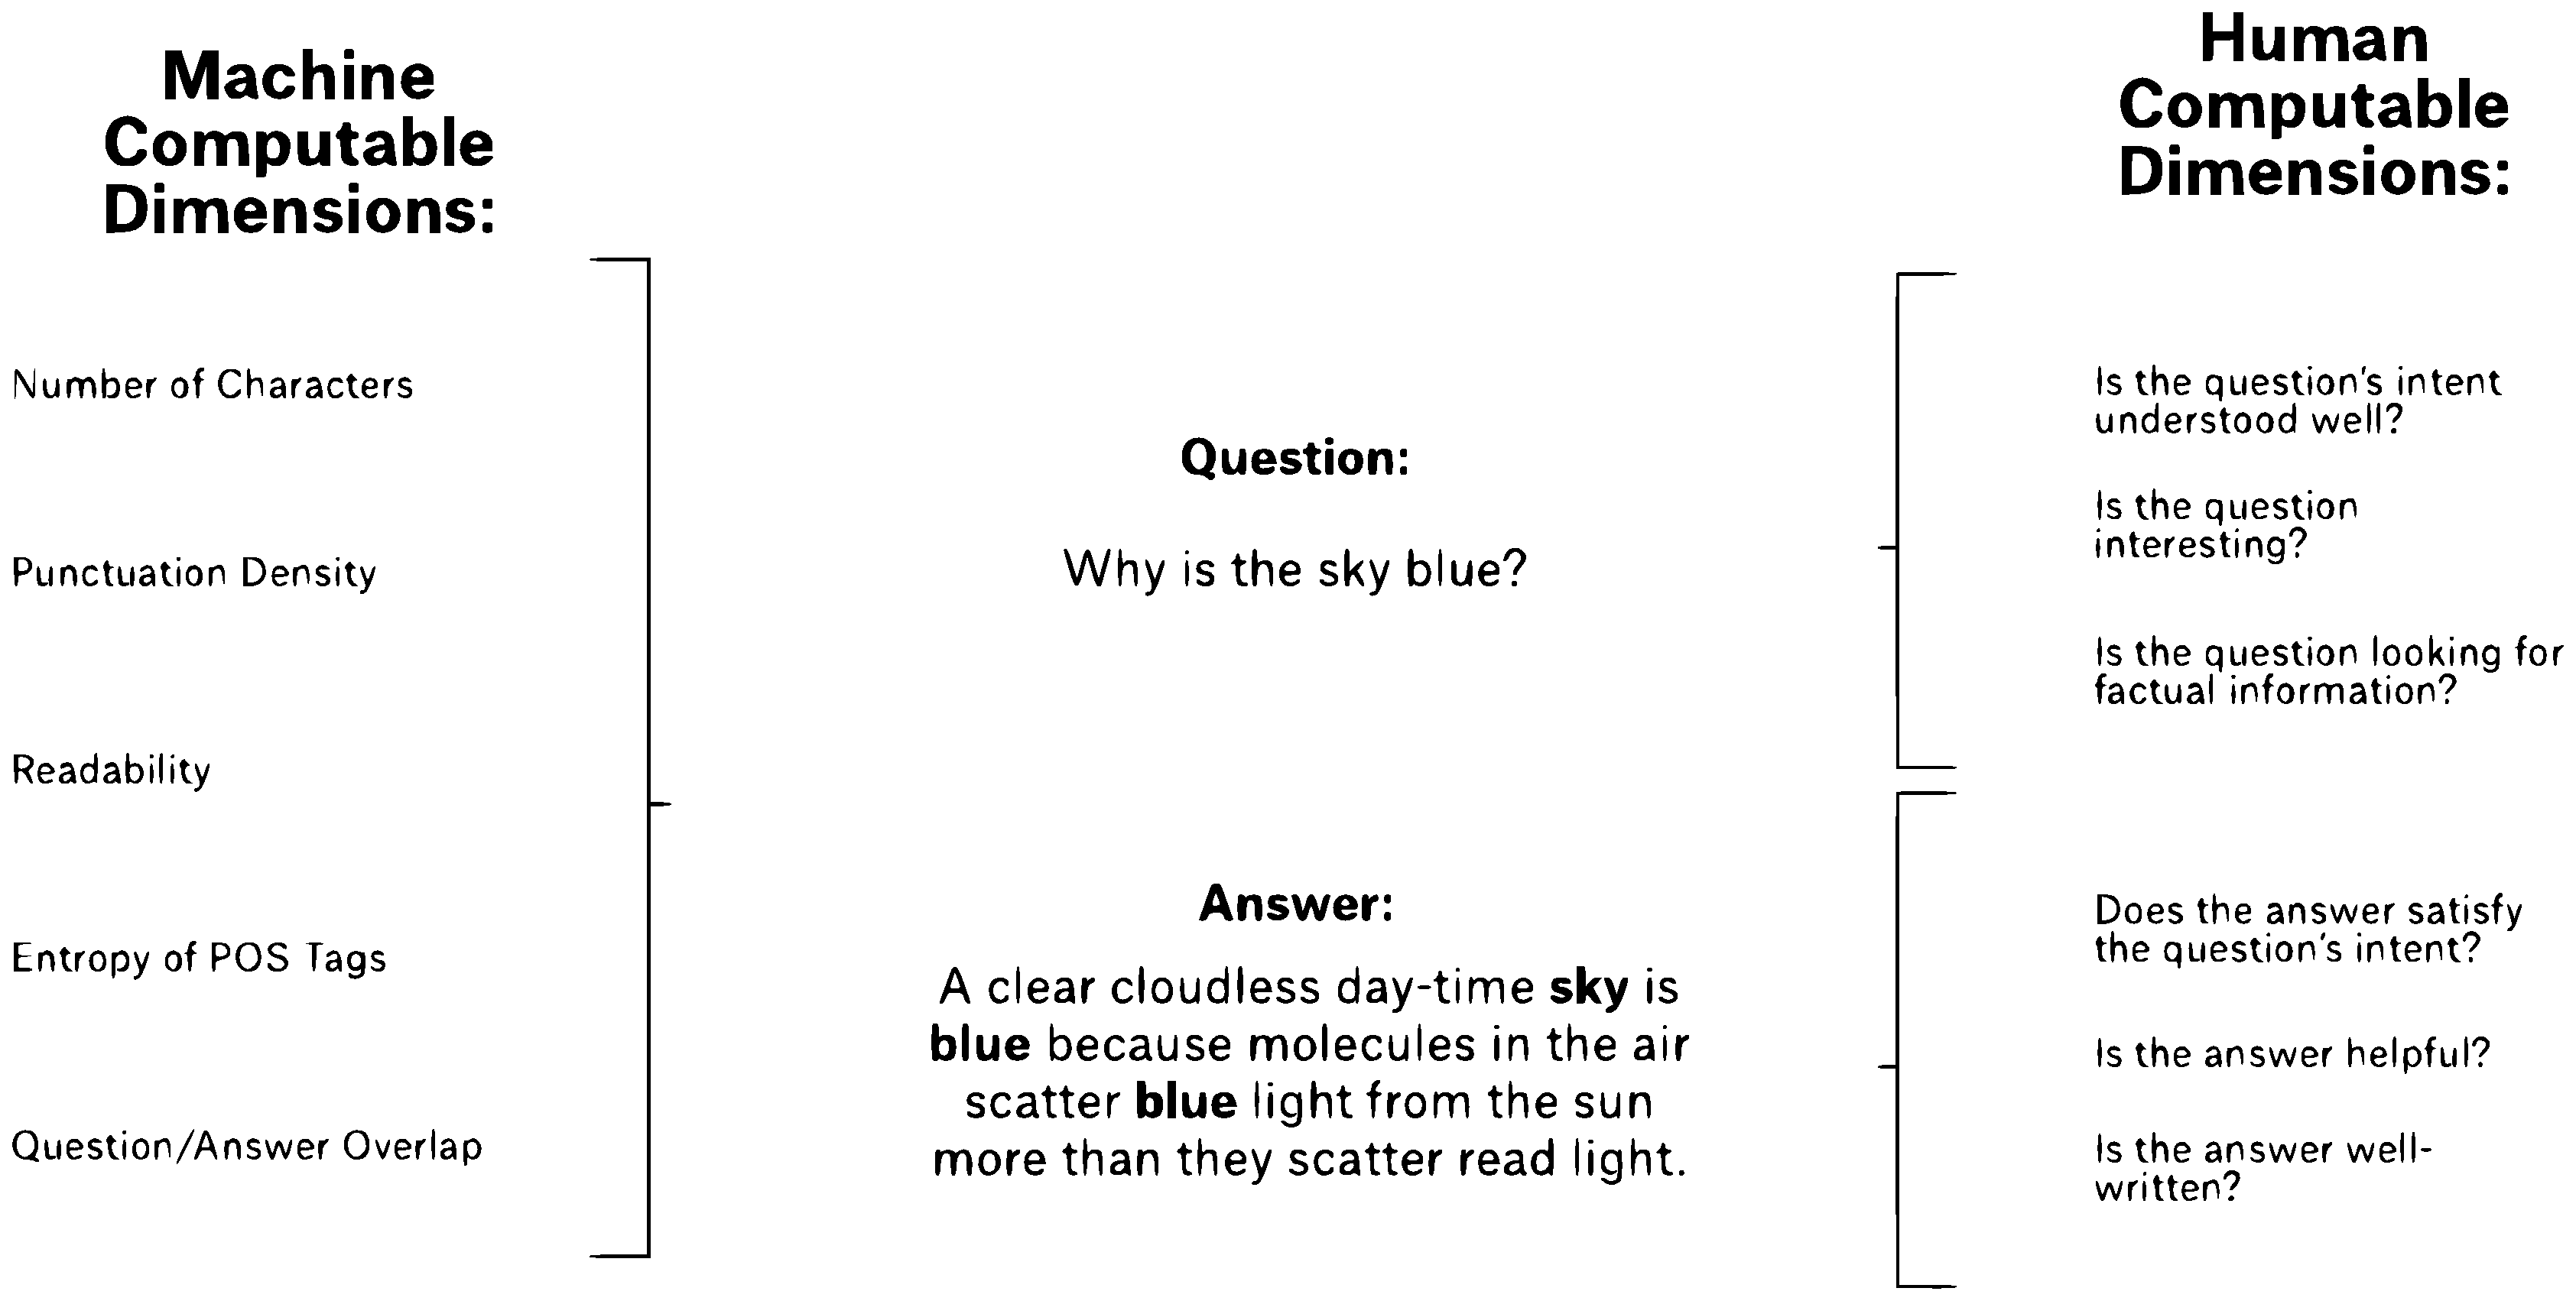
\includegraphics[width=30em]{figures/title.eps}
    \caption{Different between machine and human answer}
    \label{fig:title}
\end{figure}
\subsection{Dataset}
The dataset contains 6049 records in training set and 476 records in test set, with the following features:
\begin{itemize}
    \item Question title\&body
    \item Answer
    \item Host
    \item Category
    \item Question user
    \item Answer user
    \item Url
\end{itemize}
The targets are both continuous values in the range of $[0,1]$, representing the score of this record in the corrsponding dimension.
It contains 21 question related targets and 9 answer related targets.

\subsection{Solution}
Transformer Models such as \textit{Bert} are proven have great performance on many nlp tasks, especially for Question\&Anwser tasks.
In this competation, I will use Bert Model to solve the problem.
\newpage
\section{EDA and Data Preprocessing} \label{sec-eda}
\subsection{Host and Category}
The Q\&A pairs is collected from over 70 different web site,with 7 different category.
\begin{figure}[htbp]
    \centering
    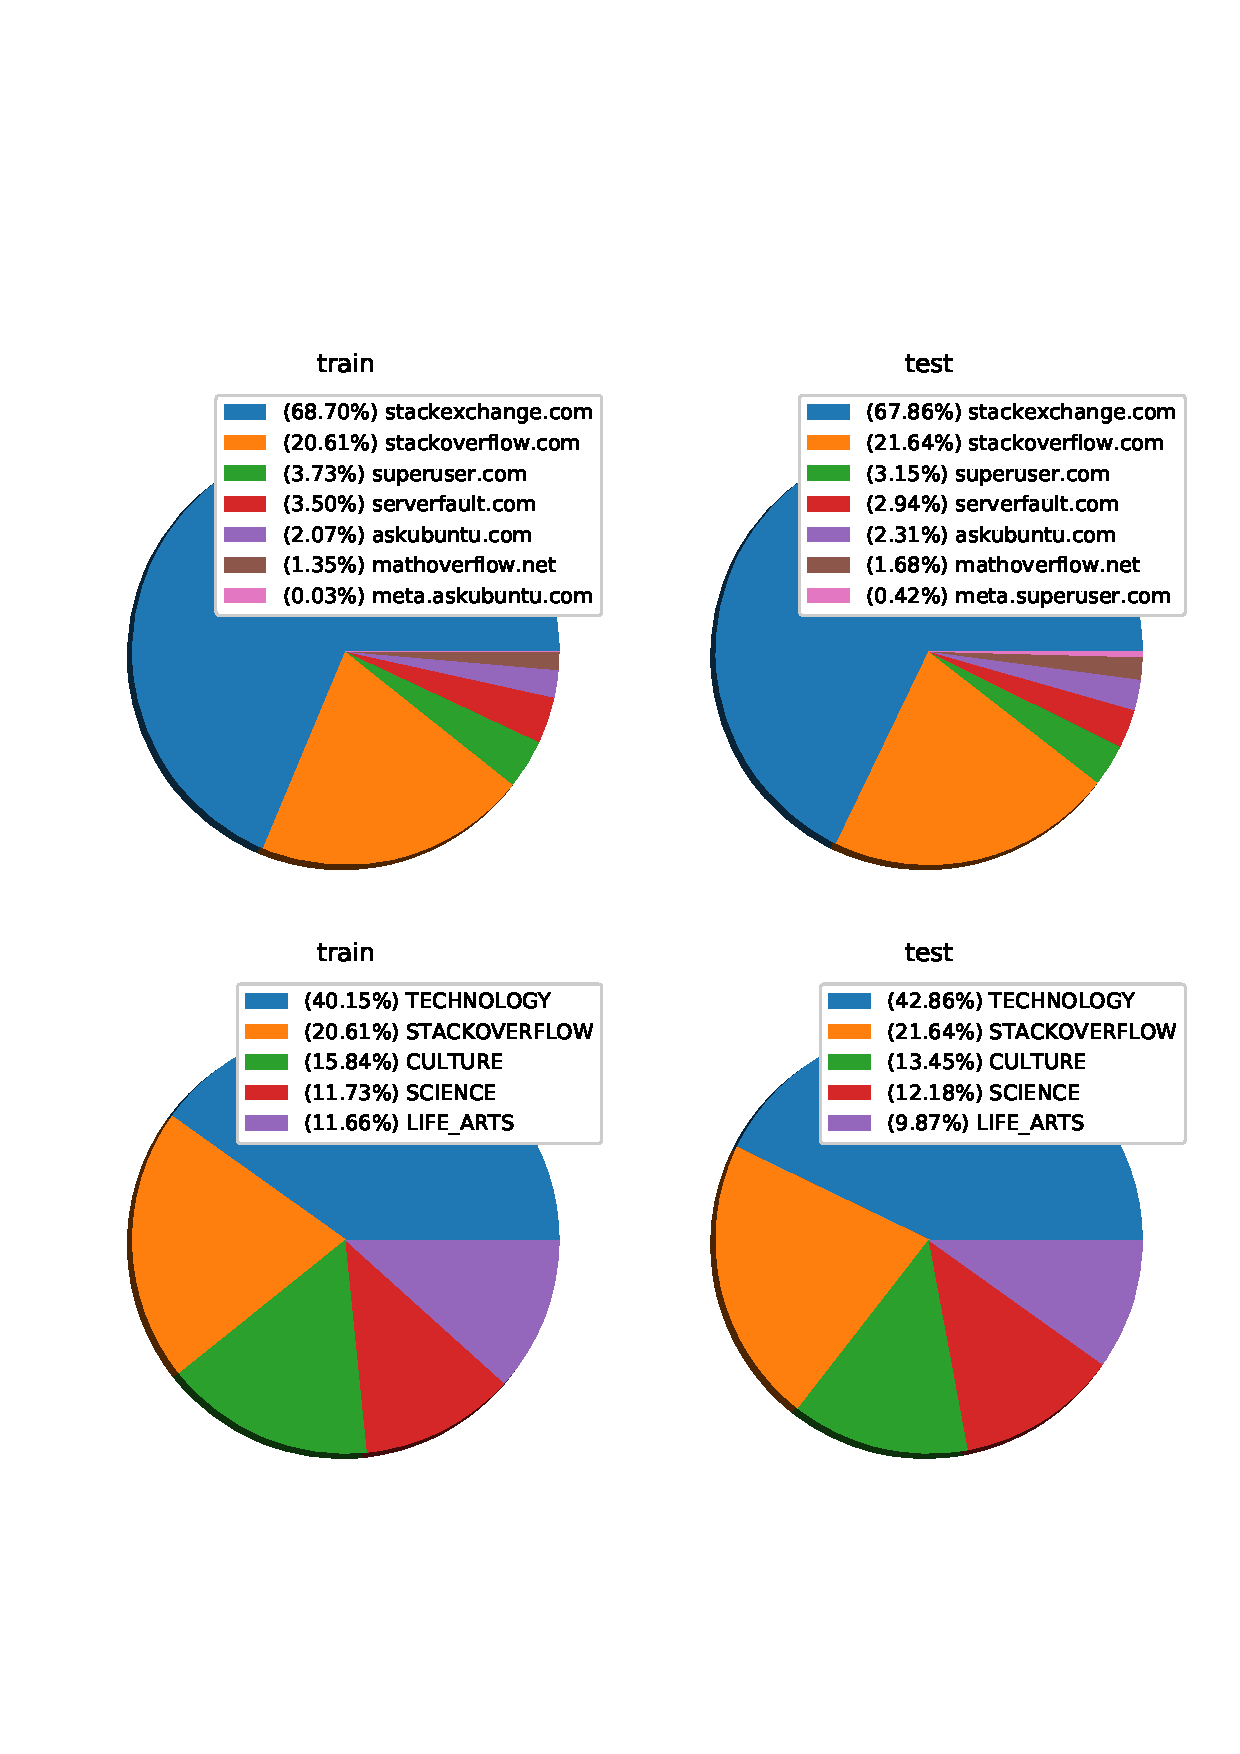
\includegraphics[width=.5\linewidth]{figures/hosts_categories.pdf}
    \caption{Category Distribution}
    \label{fig:categories}
\end{figure}
\subsection{Targets}
The 30 targets shoud be continuous values according to the competition description.
But in fact, according to the training set, they have several fixed values.
\begin{figure}[htbp]
    \centering
    \centering
    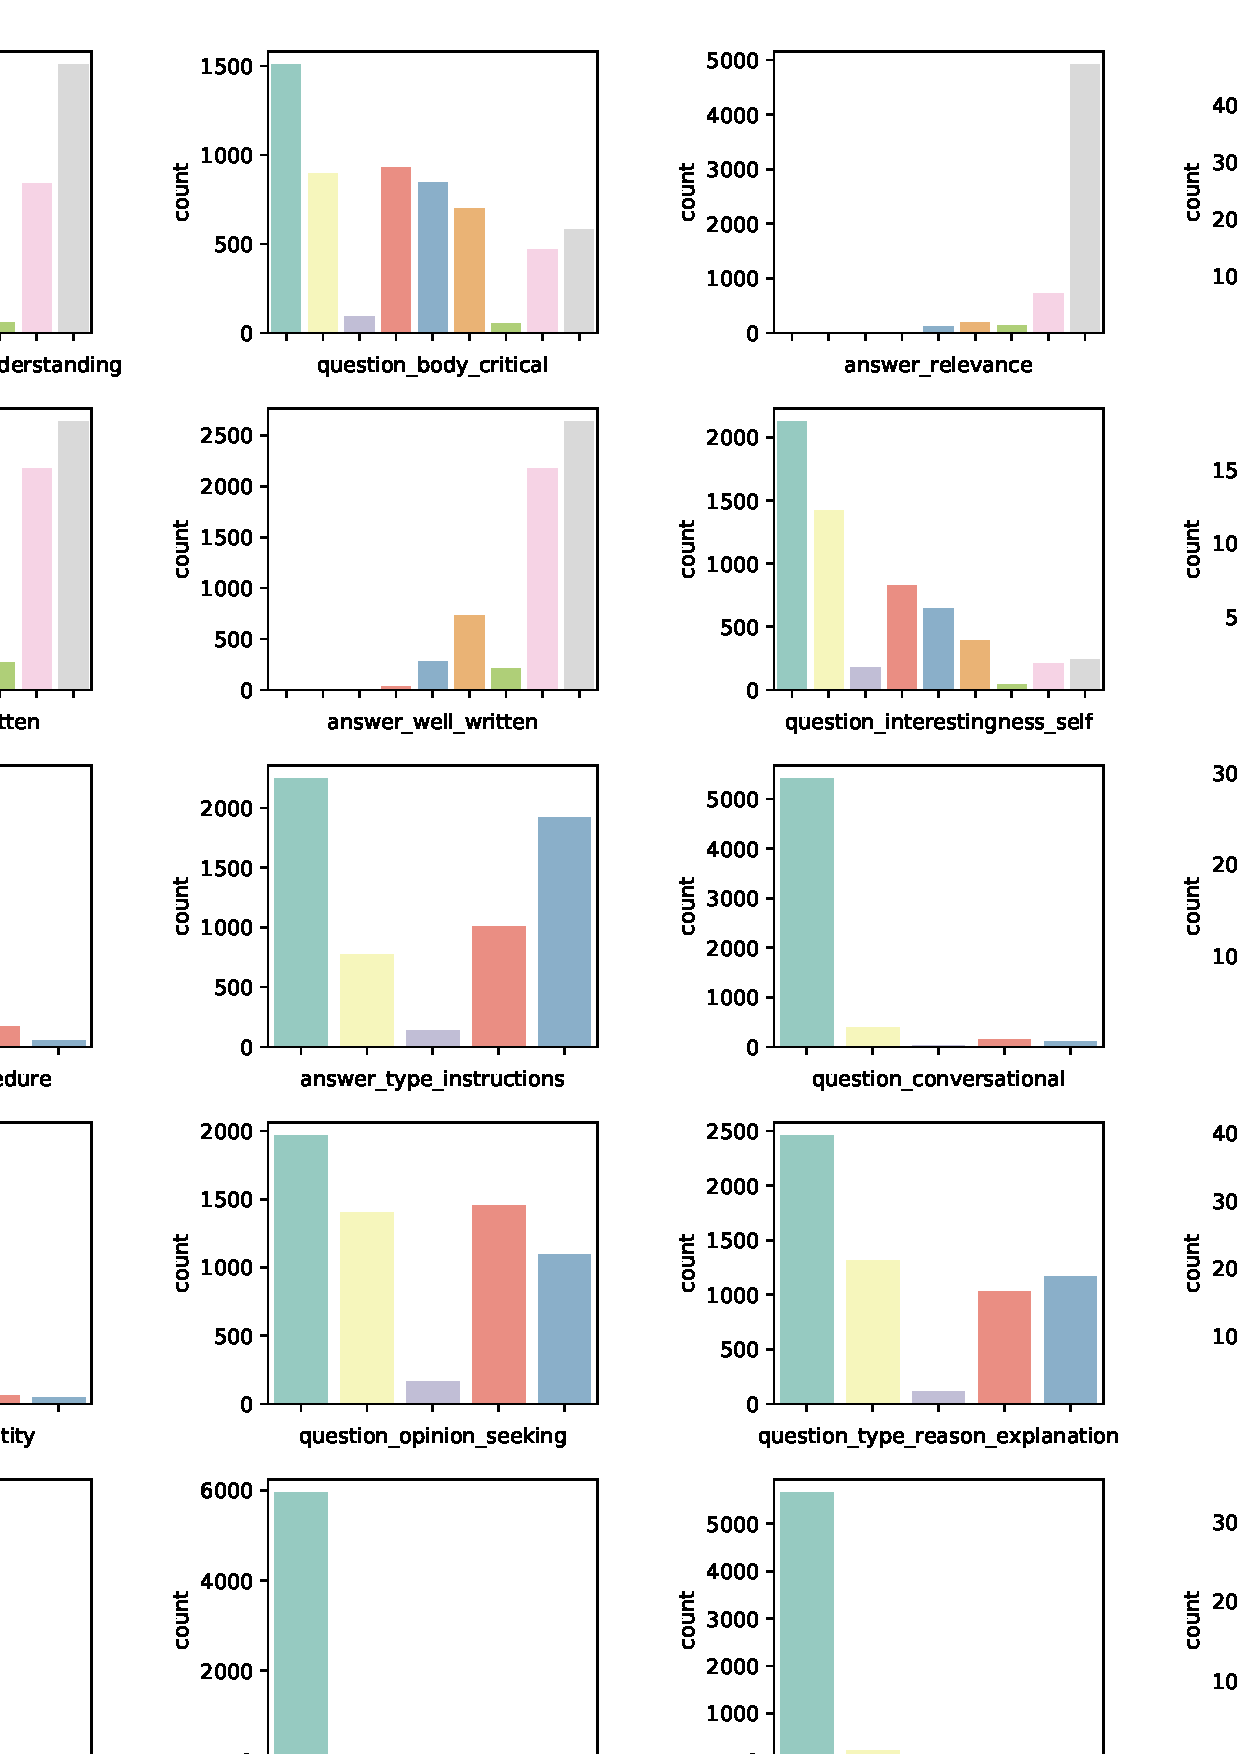
\includegraphics[width=\linewidth]{figures/targets.pdf}
    \caption{Targets Distribution}
    \label{fig:targets}
\end{figure}
\subsection{Duplicated Questions}
The competition description has said that:
\begin{itemize}
    \item \emph{The training data contains rows with some duplicated questions (but with different answers). }
    \item \emph{The test data does not contain any duplicated questions.}
\end{itemize}
\begin{table}[htbp]  
    \centering
    \caption{Duplicated Questions}
    \label{tbl:dup_q}
    \begin{tabular}{lc}
        \hline
        Question Title & Count \\
        \hline
        What is the best introductory Bayesian statist...   &12\\
        Important non-technical course for programmers?	    &11\\
        What does mathematics have to do with programm...   &11\\
        How to prevent the "Too awesome to use" syndrome    & 9\\
        How do I deal with a slow and undedicated coll...   & 7\\
        No sound in Ubuntu except at log in	                & 7\\
        What are the benefits of owning a physical book?    & 7\\
        Another instructor is pushing me out of the cl...   & 7\\
        Does "so far, so good" carry a negative connot...   & 6\\
        Good travel games for two players, especially ...   & 6\\
        \dots&-\\
        \hline
    \end{tabular}
\end{table}
\begin{itemize}
    \item The question related targets of these records are not always equle.
    \item It's reasonable to set all question related targets of duplicated questions to its mode or mean.
    \begin{itemize}
        \item \emph{t1:\ question_asker_intent_understanding}
        \item \emph{t2:\ question_body_critical}
        \item \emph{t3:\ question_conversational}
    \end{itemize}
\end{itemize}
    \begin{table}
        \centering
        \caption{The same question-related target of duplicated questions should have the same value in order to reach a better result.}
        \label{tbl:dp_before}
        \begin{minipage}{0.48\linewidth}
        \begin{tabular}{cccc}
            \hline
            qa_id	&t1 &t2 &t3 \\
            \hline
            366	    &1.00000 &1.00000 &0.00000\\
            2536	&1.00000 &1.00000 &0.66667\\
            2591	&1.00000 &1.00000 &1.00000\\
            3349	&1.00000 &1.00000 &1.00000\\
            5543	&1.00000 &1.00000 &0.00000\\
            5989	&1.00000 &1.00000 &1.00000\\
            6041	&0.77778 &1.00000 &0.66667\\
            6215	&1.00000 &0.88889 &0.33333\\
            7003	&0.77777 &1.00000 &1.00000\\
            8328	&1.00000 &1.00000 &0.66667\\
            8867	&1.00000 &1.00000 &0.66667\\
            9137	&1.00000 &1.00000 &0.00000\\
            \hline
        \end{tabular}
    \end{minipage}
    \begin{minipage}{0.48\linewidth}
        \begin{tabular}{cccc}
            \hline
            qa_id	&t1 &t2 &t3 \\
            \hline
            366	    &1.00000 &1.00000 &0.66667\\
            2536	&1.00000 &1.00000 &0.66667\\
            2591	&1.00000 &1.00000 &0.66667\\
            3349	&1.00000 &1.00000 &0.66667\\
            5543	&1.00000 &1.00000 &0.66667\\
            5989	&1.00000 &1.00000 &0.66667\\
            6041	&1.00000 &1.00000 &0.66667\\
            6215	&1.00000 &1.00000 &0.66667\\
            7003	&1.00000 &1.00000 &0.66667\\
            8328	&1.00000 &1.00000 &0.66667\\
            8867	&1.00000 &1.00000 &0.66667\\
            9137	&1.00000 &1.00000 &0.66667\\
            \hline
        \end{tabular}
    \end{minipage}
    \end{table}
\section{Method} \label{sec-method}
\subsection{Embedding}
The idea of vector semantics is thus to represent a word as a point in some multidimensional semantic space.
Vectors for representing words are generally called embeddings, because the word is embedded in a particular vector space.
After convert to embeddings, words with similar meanings are nearby in space.

There are two commonly used vector semantic models. tf-idf and word2vec.
\subsubsection{Tf-idf}
The tf-idf algorithm is the product
of two terms, each term capturing one of these two intuitions:
The first is the \textbf{term frequency}:the frequency of the word $t$ in the
document $d$. We can just use the raw count as the term frequency:
\begin{equation}
    tf_{t,d}=count(t,d)
\end{equation}
The second is used to give a higher weight to words that occur only in a
document frequency few documents,called the \textbf{inverse document frequency}. 
The document frequency $df_t$ of a term $t$ is the number of documents it occurs in.
\begin{equation}
    idf_t = \log_{10}{(\frac{N}{df_t})}
\end{equation}
Then we get the tf-idf weight value:
\begin{equation}
    w_{t,d}=tf_{d,f}\times idf_t
\end{equation}
The tf-idf vector model represents a target word as a vector with dimensions 
corresponding to all the words in the vocabulary (length $|V|$, with vocabularies of 20,000 to 50,000).
The values in each dimension are the frequency with which the target 
word co-occurs with each neighboring context word, weighted by tf-idf.
It can also be used to represent a document by the centroid document vector.
Given $k$ word vectors $w_1, w_2, \dots, w_k$, the centroid document vector $d$ is:
\begin{equation}
    d = \frac{w_1+w_2+\dots+w_k}{k}
\end{equation}
The vector can be used to estimate the similarity between the two word or documents by
compute $\cos{(d_1, d_2)}$.

\subsubsection{Word2vec}
The tf-idf vector model represent a word as a sparse, long vector. 
And it can't capture the words'position information. 
To do this, the word2vec algorithm is a better choice.
It also represent words as very short, dense vectors. 
It turn out that dense vectors work better in every NLP task than sparse vectors.

The skip-gram algorithm is one of two algorithms in a software package called word2vec,
and so sometimes the algorithm is loosely referred to as word2vec. The intuition of word2vec is that
given tuple $(t, c)$ of target word $t$ and candidate context word $c$, get whether $c$ is a real context word. (binary classification)

The intuition of skip-gram is:
\begin{enumerate}
    \item Treat the target word and a neighboring context word as positive examples.
    \item Randomly sample other words in the lexicon to get negative samples.
    \item Use logistic reg to train a classifier to distinguish those two cases.
    \item Use the reg weights as the embeddings.
\end{enumerate}
\subsection{Transformer}
\subsection{BERT}
BERT is a deep learning model that has given state-of-the-art results on 
a wide variety of natural language processing tasks. 
It stands for \textbf{Bidirectional Encoder Representations for Transformers.}
It has been pre-trained on Wikipedia and BooksCorpus and requires (only) task-specific fine-tuning.
\section{Experiment and Analysis} \label{sec-experiment}
\subsection{Model Building}
\subsection{Experiment}
\section{Conclusions} \label{sec-conclusions}


The authors would like to thank \ldots

